%!TEX root = ../proteoform_suite_manual.tex
%---------------------------------------------------------------------
%	EXPERIMENT THEORETICAL COMPARISON
%---------------------------------------------------------------------

\section{Experiment Theoretical Comparison}

\subsection{Overview}

On this page, experimental proteoforms are compared to theoretical proteoforms from the theoretical database, generating a list of experiment-theoretical pairs. Each experiment-theoretical pair has a mass difference between the experimental proteoform and the theoretical proteoform in the pair; pairs are generated for mass differences that correspond to a known set of modifications. Each experimental proteoform can be in a pair with one theoretical proteoform per protein; heuristics are used to determine the most likely pair based on the delta mass differences. A histogram is generated of the mass differences for all experiment-theoretical pairs; experiment-theoretical pairs in accepted delta mass peaks are used to construct proteoform families. Experiment-decoy pairs are generated by comparing the experimental proteoforms to the decoy databases; these pairs are used to estimate a false discovery rate for each delta mass peak. 

\subsection{Run Page}
\begin{itemize}
\item The Theoretical Proteoforms and Aggregated Proteoforms pages must be run before running this page.
\item Set all parameters as desired for current analysis (see below)
\item Click Run Page button (top right)
\item Browse the list of delta mass peaks from the histogram of experiment-theoretical pairs delta masses (top left table). Accept peaks that have an acceptable false discovery rate and correspond to common/likely modifications. For unlabeled analyses, typically only the delta mass peak closest to 0 (exact matches) is accepted. 
\end{itemize}

\subsection{Set Parameters}
\begin{figure}[h]
\centering
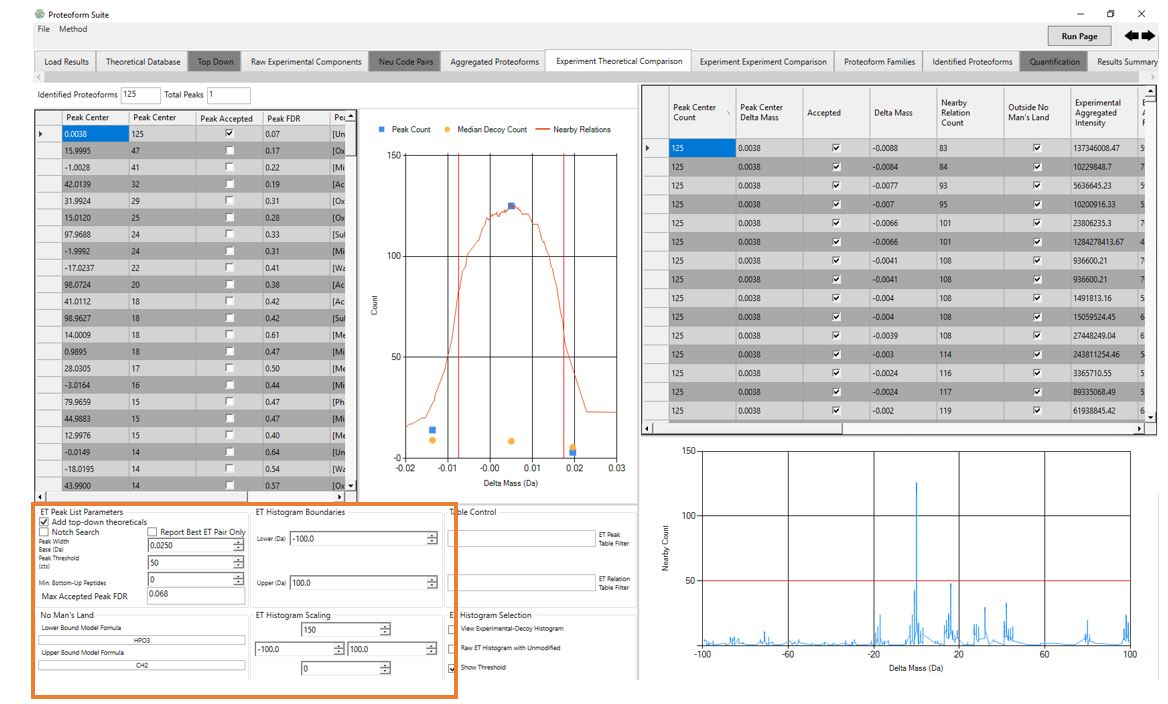
\includegraphics[scale=0.43]{figures/et1.jpg}
\end{figure}
\begin{itemize}
\item Add top-down theoreticals: if checked, theoretical proteoforms that were supplemented to the database due to the presence of a top-down proteoforms will be included in the experiment-theoretical comparison
\item Notch Search: if checked, a notch search will be performed. For each modification, experiment-theoretical pairs will be generated if the delta mass is within the set tolerance from the modification's delta mass
\item Report Best ET Pair Only: if checked, only the closest matching experiment-theoretical pair for each experimental proteoform will be included (each experimental proteoform will only be able to belong to one experiment-theoretical pair)
\item Peak Width Base (Da): if notch search is unchecked, this is the size of bins used for generating the delta mass histogram from experiment-theoretical pair delta masses
\item Peak Threshold (cts): the minimum number of experiment-theoretical pairs that must belong to a delta mass peak for the peak to be accepted
\item Min. Bottom-Up Peptides: this is the minimum number of bottom-up peptides that a theoretical proteoform must have in order to be included in the experiment-theoretical comparison. Top-down identified proteoforms are also included in the database.
\item Notch Tolerance: if a notch search is performed, this tolerance will be used to generate experiment-theoretical pairs at each modification delta mass
\item ET Histogram Boundaries: Lower (Da) and Upper (Da) delta masses to be considered for an experiment-theoretical pair to be generated 
\end{itemize}

\subsection{Results}
\begin{itemize}
	\item Identified Proteoforms: the number of accepted experiment-theoretical pairs
	\item Total Peaks: the number of accepted experiment-theoretical delta mass peaks
	\pagebreak
	\item Experiment-Theoretical Delta Mass Peaks table: the top left table displays the delta mass peaks from the histogram of experiment-theoretical pair delta masses. If a notch search is performed, each peak is a different modification delta mass/notch

	\begin{figure}[h]
\centering
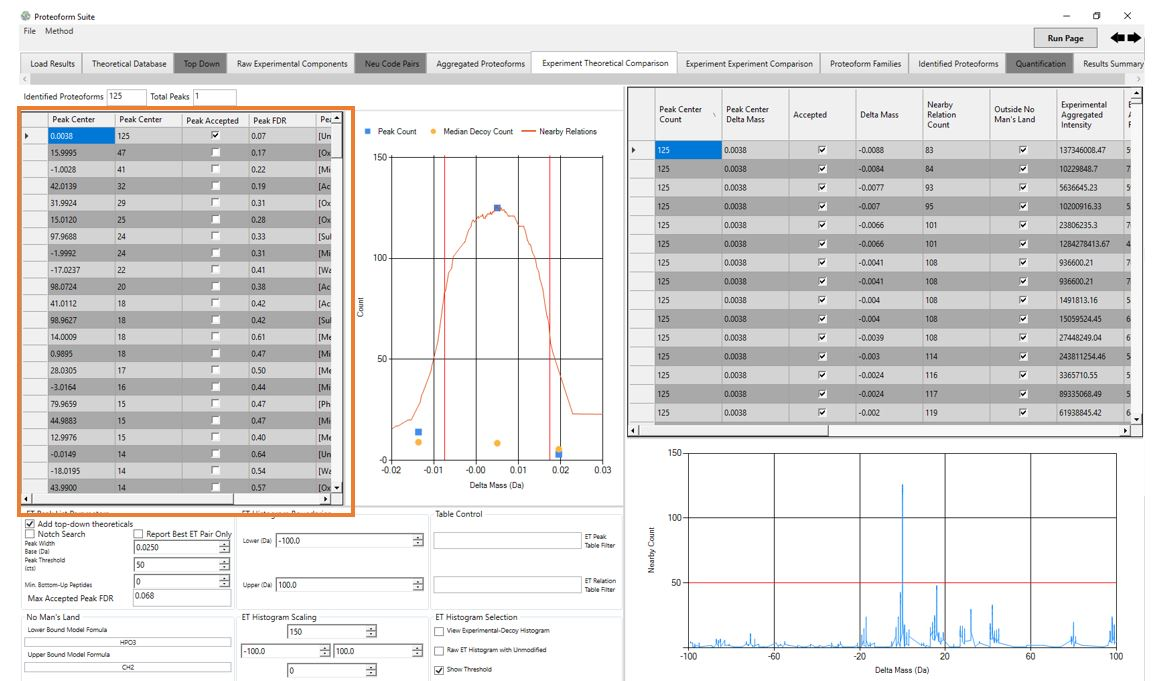
\includegraphics[scale=0.46]{figures/et2.jpg}
\end{figure}
	\begin{itemize}
		\item Peak Center Delta Mass: delta mass at the center of this delta mass peak 
		\item Peak Center Count: the number of experiment-theoretical comparisons delta masses that are part of this peak
		\item Peak Accepted: checked if peak is accepted (peak center count is above peak threshold in set parameters or manually changed by user). This check box can be checked or unchecked to accept or unaccept a delta mass peak
		\item Peak FDR: the false discovery rate for this delta mass peak; determined based on the average number of experiment-decoy pairs that fall within this peak delta mass plus/minus half of the peak width base
		\item Peak Assignment Possibilities: modifications/combinations of modifications that could correspond to the delta mass of this delta mass peak
		\item Mass Shifter: set this number to a positive or negative integer and rerun this page; the monoisotopic mass of experimental proteoforms in experiment-theoretical pairs in this peak will be shifted by the number of monoisotopic mass units of this column; useful if a peak is at a missed monoisotopic value from 0 or a modification delta mass (ex: -1 or +1 Da)
	\end{itemize}
	\item Experiment-Theoretical Delta Mass Peak Zoom-in Graph: when a peak is selected in the Experiment-Theoretical Delta Mass Peak table, this top left graph displays a zoom-in of the peak from the Experiment-Theoretical Delta Mass Histogram (bottom right graph). Blue square point is the number of experiment-theoretical pairs in the peak, and yellow circle point is median number of experiment-decoy pairs in this peak. The red line plots the nearby relations histogram count for each delta mass value
		\begin{figure}[h]
\centering
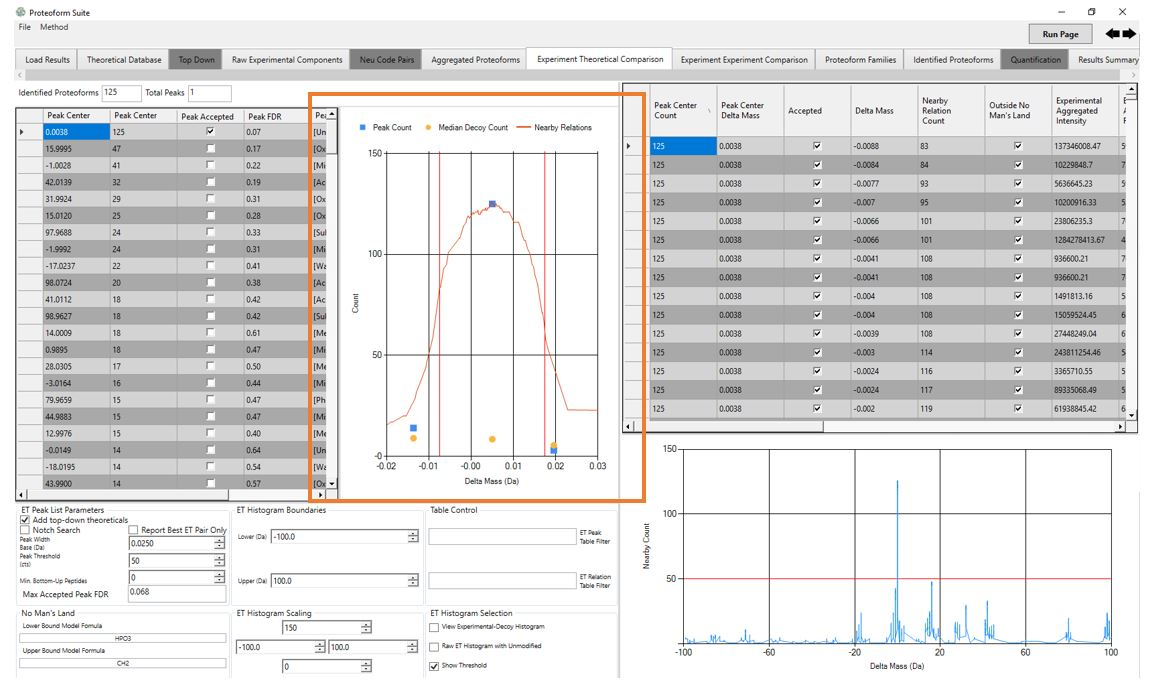
\includegraphics[scale=0.44]{figures/et3.jpg}
\end{figure}
\item {Experiment-Theoretical Pairs}: this right table displays all experiment-theoretical pairs, consisting of a theoretical proteoform, an experimental proteoform, and their mass difference.
		\begin{figure}[h]
\centering
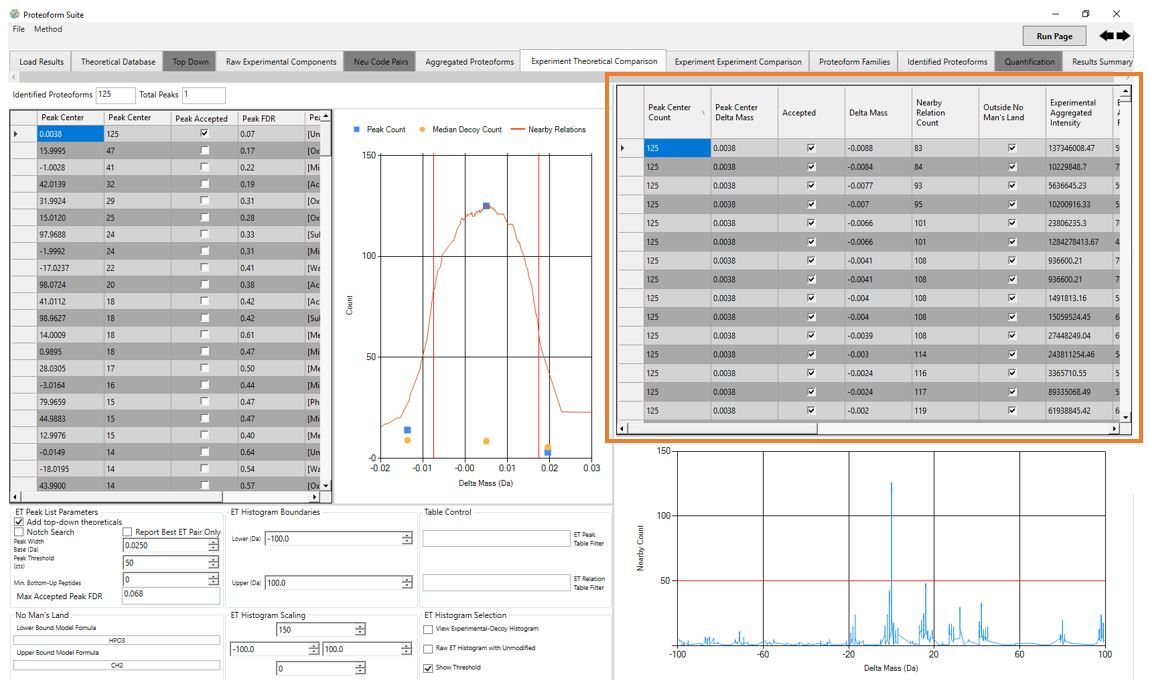
\includegraphics[scale=0.44]{figures/et4.jpg}
\end{figure}
\begin{itemize}
	\item Peak Center Count: if this pair is in a delta mass peak, the number of pairs in the peak
	\item Peak Center Delta Mass: if this pair is in a delta mass peak, the delta mass at the center of the peak
	\item Accepted: checked if this pair is in a delta mass peak that is accepted in the Experiment-Theoretical Delta Mass Peaks table
	\item Delta Mass: mass difference between the experimental and theoretical proteoform in this pair
	\item Nearby Relation Count: number of pairs with a delta mass close to this pair's delta mass; this value is used to plot the delta mass histogram
	\item Outside No Man's Land: checked if this pair is an acceptable delta mass regarding the numbers after the decimal point. Pairs with a delta mass in no man's land are not joined into delta mass peaks
	\item Experimental Aggregated Intensity: sum of intensity of aggregated raw experimental components for the experimental proteoform in this pair
	\item Experimental Aggregated RT: retention time of experimental proteoform in this pair
	\item Number Experimental Observations: number of aggregated raw experimental components (unlabeled) or NeuCode pairs (NeuCode labeled) for the experimental proteoform in this pair. If top-down proteoform, the number of top-down hits
	\item Experimental Aggregated Proteoform Mass: mass of experimental proteoform in this pair
	\item Experimental Accession: unique ID given by Proteoform Suite for experimental proteoform in this pair		
	\item Abundant Exp. Component for Manual Validation: file information for the most abundant raw experimental component aggregated into the experimental proteoform of this pair
	\item Theoretical Proteoform Mass: mass of theoretical proteoform in this pair
	\item Accession: accession given by Proteoform Suite for the theoretical proteoform in this pair
	\item Name: protein name from UniProt for the theoretical proteoform in this pair
	\item Fragment: sequence description for the theoretical proteoform in this pair
	\item Description: protein description from UniProt for the theoretical proteoform in this pair
	\item PTM Description: PTMs on theoretical proteoform in this pair
\end{itemize}
\pagebreak
\item Experiment-Theoretical Delta Mass Histogram graph: this bottom right graph shows a histogram of the delta masses for the experiment-theoretical pairs
\begin{figure}[h]
\centering
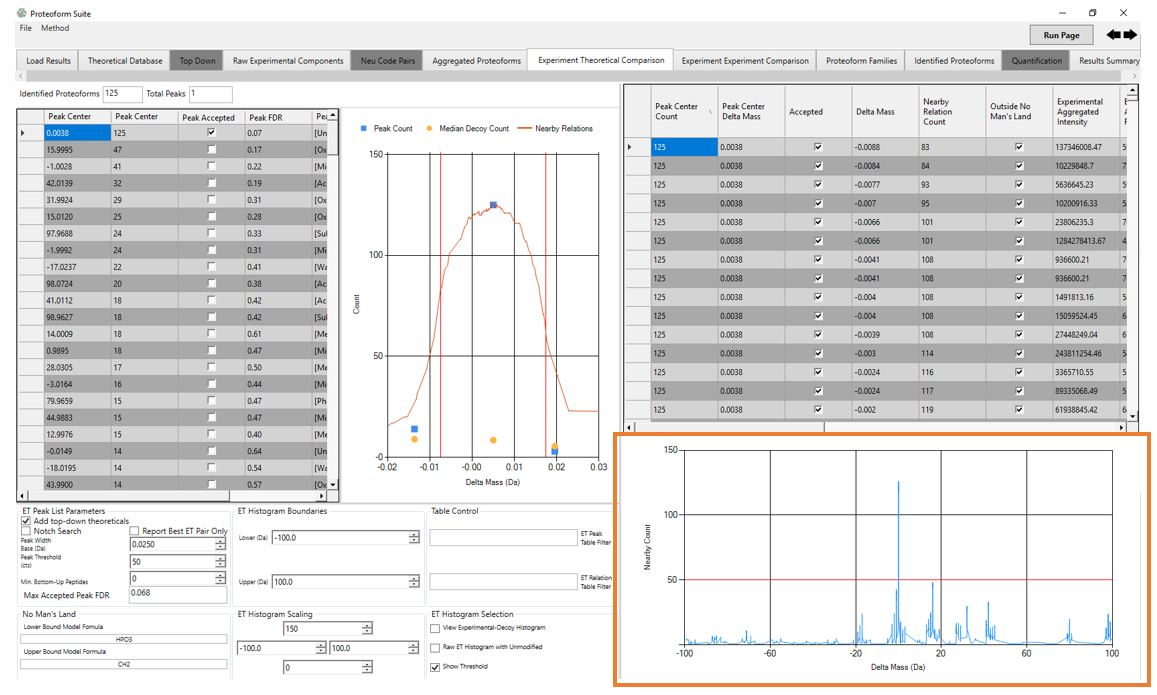
\includegraphics[scale=0.46]{figures/et5.jpg}
\end{figure}
\begin{itemize} 
	\item View Experiment-Decoy Histogram: if checked, delta mass histogram for experiment decoy pairs will be plotted
	\item Raw ET Histogram with Unmodified: if checked, a histogram with only unmodified theoretical proteoforms will be plotted using all delta mass pairs
	\item Show Threshold: if checked, a red line on the graph shows the Peak Threshold set
	\end{itemize}
\end{itemize}